\chapter{IRK: Newtonen Iterazioa.}

%\epigraph{The top 10 algorithms in Applied Mathematics: 1.Newton and quasi-Newton methods.}
%{\textit {Nick Higham (2016)}}

\section{Sarrera.}


Runge-Kutta metodo inplizituen inplementazioetan, ekuazio sistema ez-lineala modu eraginkorrean askatu behar da. Atal honetan, Newton iterazio metodoa modu eraginkorrean aplikatzeko bidea ikertuko dugu.
Problema zurruna denean, puntu finkoaren iterazio ez da eraginkorra eta Newton iterazioa aplikatu behar da. Gainera problema ez-zurruna izanik ere, Newton iterazioak interesgarriak izan daitezke; bereziki doitasun altuko (doitasun laukoitza) konputazioetan iterazio metodoaren konbergentzia ezaugarri onak direla eta. 

Ikusiko dugunez, $d$-dimentsioko ekuazio diferentzial sistema Newton iterazioan oinarritutako $s$-ataletako IRK metodoaren bidez integratzeko, era honetako ekuazio sistema lineala iteratiboki askatu behar da
\begin{equation}
\label{eq:syslin}
(I_d \otimes I_s- h \ A \otimes J) \in \mathbb{R}^{sd \times sd},
\end{equation} 
non $A \in \mathbb{R}^{s \times s}$ Runge-Kutta metodoaren koefizienteak eta $J$ matrizea, ataletan ebaluatutako Jacobiar matrizearen hurbilpen komuna den. Hau da, integrazioaren urrats bakoitzean, $sd \times sd$ tamainako ekuazio sistema lineala askatu behar da.

Lan hauetan \cite{Butcher1976} \cite{Liniger1970} \cite{Bickart1977} , (\ref{eq:syslin}) matrizearen egitura bereziari abantaila atereaz, ekuazio sistema linealak modu eraginkorrean ebazteko proposamena egin zuten. Zehazki, ia blokeka diagonala den matrizea da,  $s$-bloke $I_d-h \lambda_j J \in \mathbb{R}^{d \times d} \ (j=1,\dots,s)$, $A$ matrizearen $\lambda_j$ balio propio  bakoitzari bloke bat dagokio. Normalean, ordena altuko IRK metodoaren $A$ matrize koefizienteak, $[s/2]$ balio propio  konplexu pareak ($s$ bakoitia den kasuan balio propio erreal bat gehituta) ditu.

Gure ekarpenean, $sd$-dimentsioko ekuazio sistema (\ref{eq:syslin}) ebazteko, $(s+1)d$~dimentsioko sistema baliokidean 
berridatziko dugu, eta $d \times d$ tamainako $[s/2]+1$ matrizeen LU deskonposaketa (eta tamaina bereko matrize batzuen biderketa) kalkulatuz, askatuko dugu. Tamaina txikiko matrizeen LU deskonposaketa azkarra denez, konputazionalki eraginkorra izatea espero dugu. Algoritmoa, IRK metodoa simetriko eta sinplektikoetarako (bi propietateak betetzen dituzten metodoetarako) garatu dugu. Dena den, bai IRK metodo ez-simetriko sinplektikoetan, bai IRK metodo simetriko ez-sinplektikoetan aplika daiteke.
 
Newton iterazio metodoa, $u\in \mathbb{R}^{n}$ eta $F: \mathbb{R}^n \ \longrightarrow {\mathbb{R}}^n$ emanik, $F(u)=0$ betetzen duen $u^{[*]}$ soluzioa aurkitu nahi dugu. Hasierako soluzioaren $u^{[0]}$ estimazioa  emanik,  Newton metodoa era honetan definituko dugu (algoritmoa~\ref{alg:nssg}).

\begin{algorithm}[H]
  \BlankLine
  $ \text{Hasieratu} \ \ u^{[0]}   \quad \quad \quad \quad \quad \quad \quad \quad\quad \quad \quad \quad \quad \quad \quad \quad \quad    (64-bit)$\;
  $M=LU(J) \ \ \quad \quad \quad \quad \quad \quad \quad \quad\quad \quad \quad \quad \quad \quad \quad \quad \quad    (32-bit)$\;
  \For{ (k=1,2,\dots \text{konbergentzia lortu arte})}
  {
   \BlankLine
   $F^{[k]}=F(u^{[k-1]}) \  \quad \ \quad \quad \quad \quad \quad \quad \quad \quad \quad \quad \quad \quad \ \   (64-bit)$\;
   $\text{Askatu} \ \ M \ \Delta u^{[k]}=- F^{[k]} \ \quad \ \quad \quad \quad \quad \quad \quad \quad \quad \ \ \  (32-bit)$\;
   \BlankLine
   $u^{[k]}=u^{[k-1]}+\Delta u^{[k]}  \ \ \ \quad \quad \quad \quad\quad \quad \quad \quad \quad \quad \quad \ \     (64-bit)$\;
  }
 \caption{Newton sinplifikatua.}
 \label{alg:nssg}
\end{algorithm}

non $J \in \mathbb{R}^{n \times n}$, $J^{[k]}=J(u^{[k]})$ matrize Jacobiarraren hurbilpena den,
\begin{equation*}
J(u^{[k]})=(J_{ij}(u^{[k]}))_{i,j}^n \ \text{non} \ J_{ij}(u^{[k]})=\partial f_i/\partial u_j (u^{[k]}), \ \ 1 \leq i,j \leq n. 
\end{equation*} 


Azpimarratzekoa da ere, Newton metodoaren eragiketa konplexuenak doitasun txikiagoan kalkula daitezkeela \cite{Baboulin20092526} eta honek, konputazionalki abantaila interesgarria suposatzen duela. Algoritmoaren (Algoritmoa \ref{alg:nssg}) eskubi aldean, doitasun bikoitzeko ($64$-bit) inplementazioa balitz, eragiketa bakoitzaren doitasuna zehaztu dugu: Jacobiarraren balioztapena eta aljebra linealeko eragiketak, doitasun arruntean ($32$-bit) kalkulatu daitezke.


\section{IRK-Newton estandarra.}

\paragraph*{}Demagun honako hasierako baliodun problema,
\begin{equation}
\label{eq:hbp}
\dot{y}=f(t,y),\ \ \ y(t_0)=y_0, 
\end{equation}
non  $y_0 \in \mathbb{R}^{d}$  eta $f: \  {\mathbb{R}}^{d+1} \ \longrightarrow {\mathbb{R}}^d$ diren. 

\paragraph*{}Denbora diskretizazioa $t_0<t_1<t_2<\dots$ emanik, (\ref{eq:hbp}) hasierako baliodun problemaren $y(t)$ soluzioaren $y_n \approx y(t_n), (n=1,2,\dots)$ zenbakizko soluzioa, integrazio metodo bat aplikatuz
\begin{equation}
y_{n+1}=\Phi(y_n, t_n, t_{n+1}-t_n),
\end{equation}
lortuko dugu, non $\Phi:\mathbb{R}^{d+2} \rightarrow \mathbb{R}$ den.

\paragraph*{}S-ataletako IRK metodoaren kasuan,  $a_{ij}, b_i, \ \text{eta} \ c_i \ (1\leqslant i,j \leqslant s)$ koefizienteek definitzen dute $\Phi$ integrazio metodoa,
\begin{equation}  
\label{eq:irkn1}
\Phi(y,t,h)=y+h\sum^s_{i=1}{b_i \ f(t_+c_ih,Y_{i})\ \ },\
\end{equation} 

non $c_i=\sum_{j=1}^{s} a_{ij}$ izan ohi da eta $Y_{i}$ atalak era honetan inplizituki  definitzen diren,
\begin{equation}
\label{eq:irkyi}
Y_{i}=y+\ h\ \sum^s_{j=1}{a_{ij}\ f(t+c_jh,Y_{j})}\ \ \ \ \ i=1 ,\dots, s.\
\end{equation} 

$Y_{i} \in \mathbb{R}^d,\ i=1,\ldots,s$ ezezagunen eta $sd$ tamainako ekuazio sistema ez-lineala (\ref{eq:irkyi}) askatzeko, iterazio metodo bat aplikatu behar dugu. Aurreko atalean puntu-finkoaren iterazioa aztertu genuen eta atal honetan,  Newton iterazio metodoa modu eraginkorrean aplikatzeko bidea ikertuko dugu.

%Newton iterazio bakoitzean, $\partial f/ \partial y$ matrize jacobiarraren $s$ ebaluazio eta $sd \times sd$ tamaineko  matrizearen LU deskomposaketa kalkulatzea beharrezkoa da, eta beraz konputazionalki merkeagoak diren aldaerak erabili ohi dira.

\subsection*{Newton iterazioa.}

Newton $k=1,2,\dots$ iterazioetarako, (\ref{eq:irkyi}) ekuazio inplizituko $Y_i \ (i=1,\dots,s)$ atalen  $Y_i^{[k]}$ hurbilpenak kalkulatzeko algoritmoa, modu honetan definituko dugu,

\begin{align}
\label{eq:(1)Newton_iteration}
1) & \quad r_i^{[k]} := -Y_{i}^{[k-1]} + y + h \sum_{j=1}^{s}\, a_{ij}\, f(t + c_j h,Y_{j}^{[k-1]}), \quad  i=1 ,\ldots, s, \\
\label{eq:(2)Newton_iteration}
\begin{split}
2) & \quad \mathrm{Askatu \ } \Delta Y_{i}^{[k]},\\
& \quad \Delta Y_{i}^{[k]}  - h \sum_{j=1}^{s}\, a_{ij}\, J_j^{[k]} \Delta Y_{j}^{[k]} = r_i^{[k]} \quad  i=1 ,\ldots, s, \\
& \mbox{non} \quad  J_i^{[k]}=\frac{\partial f}{\partial y}(t + c_i h,Y_{i}^{[k]}) \quad \quad  i=1,\ldots, s, 
\end{split} \\
\label{eq:(3)Newton_iteration}
3)& \quad Y_i^{[k]} := Y_i^{[k-1]} + \Delta Y_i^{[k]}, \quad  i=1 ,\ldots, s,
\end{align}

\paragraph*{}Azpimarratu behar da iterazio bakoitzeko,  $J_i^{[k]}$ Jacobiarraren $s$ ebaluazio eta $sd \times sd$ tamainako matrizearen LU-deskonposaketa kalkulatu behar ditugula. Eragiketa hauek konplexuak dira eta horregatik, Newton osoaren inplementazioa konputazionalki oso garestia da. Aukera eraginkorragoen artean, bi aipatuko ditugu:

\begin{enumerate}
\item Newton interazio sinplifikatuak aplikatzea. 
Aukera honetan, (\ref{eq:(2)Newton_iteration}) ekuazioaren $J_i^{[k]}$ Jacobiar matrizeak, $J_i^{[0]}=\frac{\partial f}{\partial y}(t+c_ih, Y_i^{[0]})$ matrizeekin ordezkatuko dira. Era honetan, urratsero behin bakarrik egin beharko litzateke LU deskonposaketa.

\item (\ref{eq:(2)Newton_iteration}) ekuazio sistema,  aurrebaldintzatutako  matrize honen
\begin{equation}
\label{eq:irksys}
(I_s \otimes I_d - h \ A \otimes J)
\end{equation}
alderantzizkoarekin iterazio metodoaren \cite{Saad2003} bidez ebaztea.
\end{enumerate}

Dena dela, goiko bi aukeretan era honetako ekuazio sistemak askatu behar dira,
\begin{equation}
(I_d \otimes I_d - h \ A \otimes J) \ \Delta Y = r )
\end{equation} 
emandako $r \in R^{sd}$ izanik. Ekuazio sistema $sd \times sd$ tamainako matrize osoaren LU deskonposaketa eginez ebatzi daiteke baina modu eraginkorragoan egiteko bideak aztertuko ditugu.

\paragraph*{}Modu estandarrenean  \cite{Butcher1976} \cite{Liniger1970} \cite{Bickart1977} , $A$ matrizearen diagonalizatzen da $\Lambda = S^{-1} A S=\mathrm{diag}(\lambda_1,\ldots,\lambda_s)$ eta era honetako matrizearen,
\begin{equation*}
I_s \otimes I_\dim  - h \, \Lambda \otimes J = (S^{-1} \otimes I_\dim) \left( I_s \otimes I_\dim  - h \, A \otimes J\right) (S \otimes I_\dim)
\end{equation*}
LU deskonposaketa kalkulatuko da. $A$ matrizearen balio propio erreal bakoitzari dagokion $d \times d$ matrize errealen LU deskonposaketak kalkulatu behar dira.

Beste autore batzuk \cite{Brugnano2014} \cite{Jay2009}, (\ref{eq:irksys}) ekuazio sistema askatzeko, matrize alderantzizko honen,
\begin{equation}
I_d \otimes I_s -h \ \bar{A} \otimes J,
\end{equation}
non $\bar{A} \in \mathbb{R}^{s \times s}$ (LU deskonposaketa modu eraginkorragoan askatzeko aukeratua) aurrebaldintzatutako iterazioa aplikatzea proposatzen dute. 


\subsection*{Newton sinplifikatuaren iterazioa.}

Newton sinplifikatuaren iterazioa aplikatzerakoan, $J_i^{[k]}$ Jacobiarrak,  $J_i^{[0]}=\partial f / \partial y \ (t+c_ih, Y_i^{[0]}) \ \ i=1,\cdots,s$ Jacobiarrekin ordezkatzen dira eta orduan, askatu beharreko ekuazio sistema honakoa da,
\begin{equation*}
\Delta Y_{i}^{[k]}  - h \sum_{j=1}^{s}\, a_{ij}\, J_j^{[0]} \Delta Y_{j}^{[k]} = r_i^{[k]}, \quad  i=1 ,\ldots, s,
\end{equation*}
non $\quad  J_i^{[0]}=\frac{\partial f}{\partial y}(t + c_i h,Y_{i}^{[0]}), \quad  i=1,\ldots,s \ $ den.

Lehen sinplifikazio honetan, integrazioaren urrats bakoitzeko,  $J_i^{[0]}$ Jacobiarraren s-ebaluazio eta $sd \times sd$ tamainako matrizearen LU deskonposaketa behin bakarrik kalkulatu behar ditugu. Modu baliokidean, ekuazio lineala notazio matriziala erabiliz laburtu daiteke,
\begin{equation*}
\label{eq:805}
\left (I_s \otimes I_d - h  
\begin{bmatrix}
a_{11}  J_1^{[0]} & \dots & a_{1s}  J_s^{[0]} \\
a_{21}  J_1^{[0]} & \dots & a_{2s}  J_s^{[0]} \\
\vdots            & \ddots & \vdots \\
a_{s1}  J_1^{[0]} & \dots & a_{ss}  J_s^{[0]} \\ 
\end{bmatrix} \right) \Delta Y^{[k]} =r^{[k]}.
\end{equation*}

non,
\begin{equation*}
\label{eq:806}
Y^{[k]}=\begin{bmatrix}
Y_1^{[k]} \\
\vdots \\
Y_s^{[k]}
\end{bmatrix} \in \mathbb{R}^{sd}, \ \ \
r^{[k]}=\begin{bmatrix}
r_1^{[k]} \\
\vdots \\
r_s^{[k]}
\end{bmatrix} \in \mathbb{R}^{sd},
\end{equation*}

\begin{equation*}
\label{eq:807}
J_{is}(y)=\left(\partial f^i/\partial y^j (y)\right)_{i,j}^d=
\begin{bmatrix}
    \frac{\partial f^1}{\partial y^1} & \cdots & \frac{\partial f^1}{\partial y^d}\\    
    \vdots & \ddots & \vdots \\    
    \frac{\partial f^d}{\partial y^1} & \cdots & \frac{\partial f^d}{\partial y^d}\\    
\end{bmatrix} \in \mathbb{R}^{d \times d},\ is=1,\cdots,s.
\end{equation*}

\subsection*{Newton super-sinplifikatuaren iterazioa.}

Bigarren sinplifikazioa bat aplika daiteke, $J_i^{[0]}=\partial f / \partial y \ (t+c_ih, Y_i^{[0]}), \ \  i=1,\dots,s \ $ matrizeak,  $J_i^{[0]} \approx J$ hurbilpen bakarrekin ordezkatuz. Era honetako ekuazio sistema lortuko dugu,   

\begin{equation}
\label{eq:808}
(I_s \otimes I_d - h \ A \otimes J) \Delta Y^{[k]} = r^{[k]}.
\end{equation}
non $I_s,I_d$ identitate eta $A=(a_{ij})_{i,j}^s$ koefizienteen matrizeak diren.

Problema zurruna denean, atalen hasieraketa $Y_i^{[0]}=y_n, \ i=1,\dots,s$  erabili ohi da, eta Jacobiarraren hurbilpen honekin $J=\partial f / \partial y \ (t+h/2, y_n)$, ekuazio lineala askatzeak zentzua izango du.  Aukera egokia da ere~\cite{Xie2009},  $J=  \frac{\partial f}{\partial y}(t+\bar c \, h,\bar y)$ aplikatzea, non $\bar c = \frac{1}{s} \sum_{i=1}^{s}c_i$ (metodo simetrikoetan $\bar c = \frac12$ da)  eta  $\bar y =  \frac{1}{s} \sum_{i=1}^{s}Y_i^{[0]}$. Maiz, $\partial f/\partial y$  konputazionalki merkeagoa den hurbilketa batez ordezkatzea nahikoa izango da. 

Newton iterazio bertsio honi super-sinplifikatua deitu diogu. Iterazio bakoitzean $f$ funtzioaren $s$ ebaluazio eta $sd$ dimentsioko ekuazio-sistema lineala askatu behar da. $(I_s \otimes I_d - h \ A \otimes J)$ matrizea iterazio guztietarako berdina da,  bere LU deskonposaketa behin bakarrik egin behar da baina konputazionalki garestia da \cite{Butcher1976} \cite{Hairer1996}. Hau da aljebra linealari dagokion eragiketen konplexutasuna,
\begin{align*}
&\text{LU deskonposaketa}, \ \ 2s^3d^3/3+\mathcal{O}(d^3), \\
&\text{back substitution}, \ \ 2s^2d^2+\mathcal{O}(d).
\end{align*}

Jarraian, Newton super-sinplifikatuaren inplementazioaren algoritmo orokorra laburtu dugu (Algoritmoa \ref{alg:nss}).

\subsection*{Algoritmoa.}

\begin{algorithm}[H]
 \BlankLine
  $\tilde{y}_0=fl(y_0)$\;
  $e_0=fl(y_0-\tilde{y}_0)$\;
  \For{$n\leftarrow 0$ \KwTo ($endstep-1$)}
  {
   \BlankLine
   $k=0$\;
   \text{Hasieratu} $Y_{n,i}^{[0]} \ \ , \ \ i=1,\dots,s $\;
   \BlankLine
   $J=\frac{\partial f}{\partial y}(t+h/2,y_n) $\; 
   $M=LU(I_s \otimes I_d - h \ A \otimes J)$\;
   \BlankLine
   \While{ (\text{not konbergentzia})}
   {
    \BlankLine 
    $k=k+1$\;
    $r_i^{[k]}=-Y_{n,i}^{[k-1]}+y_n+\big(e_n+h \sum\limits_{j=1}^{s} a_{ij} f(t+c_jh,Y_{n,j}^{[k-1]})\big) $\;
    \text{Askatu} $(M \Delta Y_n^{[k]}=r^{[k]})$\;
    $Y_n^{[k]}=Y_n^{[k-1]}+\Delta Y_n^{[k]}$\;
    $\text{konbergentzia} \leftarrow \text{GeratzeErizpidea}(Y_n^{[k]},Y_n^{[k-1]},\Delta_{min}) $\;
   }
   \BlankLine
   \If{($\exists j \ \text{non} \ \Delta_j^{[K]}\neq 0$)}
   {
    \If{$(NormalizeDistance(Y_n^{[k]},Y_n^{[k-1]})>1$}
     {$\text{fail convergence}$\;}
   }
   {$(\tilde y_{n+1},e_{n+1})\leftarrow \text{baturakonpensatua}(y_n,e_n,Y_n^{[k]})$\;}    
 }
 \caption{IRK (Newton super-sinplifikatua).}
 \label{alg:nss}
\end{algorithm}



\section{IRK-Newton eraginkorra.}
\label{sec:s74}

\subsection{Ekuazio-sistema.}

Atal honetan, honako ekuazio lineala modu eraginkorrean askatzeko inplementazioa proposatuko,
\begin{equation}
\label{eq:linsys}
(I_s \otimes I_d - h \ A \otimes J) \ \Delta Y = r,
\end{equation}
non $J \in \mathbb{R}^{d \times d}$  eta $r \in \mathbb{R}^{s \times d}$ emandako matrizeak izanik.

\paragraph*{}$S$-ataletako IRK metodoa, Newton iterazioaren bidez $d$-dimentsioko ODE sistemari aplikatzeko, urrats bakoitzean $sd \times sd$ tamainako hainbat ekuazio sistema (iterazio bakoitzeko bat) askatu behar dira. Atal honetan, jatorrizko $sd$-dimentsioko ekuazio- sistema, $(s+1)d$ dimentsioko ekuazio-sistema baliokide moduan berridatziko dugu. Ekuazio-sistema baliokide hau,  $d \times d$ tamainako $[s/2]+1$ matrize errealen LU deskonposaketa bidez askatuko dugu. Tamaina txikiko matrizeen LU deskonposaketa azkarra denez, konputazionalki eraginkorragoa izatea espero dugu.      

\paragraph*{}Gauss nodoetan oinarritutako \emph{RK} kolokazio metodoak, sinplektikoak eta simetrikoak \cite{Sanz-Serna1992} dira. 
\begin{enumerate}
\item Sinplektikoa.

Runge-Kutta metodoa sinplektikoa izateko baldintza,
\begin{equation} 
\label{eq:sympl}
b_{i}a_{ij}+b_{j}a_{ji}-b_{i}b_{j}=0, \ \ 1 \leqslant i,j \leqslant s.
\end{equation} 
\item Simetrikoa.

Runge-kutta metodoa simetrikoa izateko baldintza,
\begin{align}
\label{eq:simm}
\begin{split}
b_{s+1-i}=b_i, \ \ {c}_{s+1-i}=1-{c}_i,& \quad \ 1\leqslant i,j \leqslant s, \\
b_j={a}_{s+1-i,s+1-j}+a_{i,j},& \quad 1\leqslant i,j \leqslant s. 
\end{split}
\end{align} 
\end{enumerate}

Bi propietate hauetan oinarrituko gara inplementazio eraginkorra garatzeko.

S-ataletako IRK metodoa (\ref{eq:irkn1}), baliokidean den modu honetan berridatzi daiteke,
\begin{equation}
\Phi(y,t,h):=y+z,
\end{equation}
non $Y_i \in \mathbb{R}^d$ atalak eta $z \in \mathbb{R}^d$ gehikuntza, inplizituki era honetan definitzen diren,
\begin{align}
&Y_{i}=y+\frac{z}{2}+ h\ \sum^s_{j=1}{\bar{a}_{ij}\ f(t+c_jh,Y_{j})}\ \ \ \ \ i=1 ,\dots, s,\\
&z=h \sum_{i=1}^{s} {b_i \ f(t+c_ih,Y_{i})},
\end{align} 
non
\begin{equation}
\bar{a}_{ij}=a_{ij}-\frac{b_j}{2}, \quad 1\leqslant i,j \leqslant s \ \ \text{den}.
\end{equation} 

Ekuazio inplizitua ebazteko Newton iterazio sinplifikatua aplikatzen badugu, $(s+1) \times d$ dimentsioko ekuazio-sistema askatu behar dugu,
\begin{align}
\label{eq:linsys2}
\begin{split}
(I_s \otimes I_d- h \ \bar{A} \otimes J) \ \Delta Y - \frac{1}{2}(e_s \otimes I_d) \ \Delta z =r,\\
(-h e_s^T B \otimes J) \ \Delta Y+  \Delta z=0,
\end{split}
\end{align}
non $e_s=(1,\dots,1)^T \in \mathbb{R}^{s}, \ \text{eta} \ \bar{A}=(\bar{a}_{ij})_{i,j=1}^s$ den. Argi dago, $(\Delta Y, \Delta z)$ ekuazio-sistema honen (\ref{eq:linsys2}) soluzioa bada, orduan $\Delta Y$ gure jatorrizko ekuazio sistemaren (\ref{eq:linsys}) soluzioa dela.

\paragraph*{} Ekuazio-sistemaren adierazpen matriziala lagungarria izan daiteke,
\begin{equation*}
\begin{bmatrix}
    &      &      &  & \ \ -I_d/2 \\
    &      &      &  & \ \ -I_d/2 \\
    &      &      &  & \ \      \\    
    &  & I_s \otimes I_d- h \ \bar{A} \otimes J & & \ \ \vdots \\
    &      &      &  & \ \      \\
    &      &      &  & \ \ \ \ -I_d/2    \\
-hb_1 J & -hb_2 J & \dots & -hb_s J &  I_d\\ 
\end{bmatrix}
\begin{bmatrix}
\Delta Y_1 \\
\Delta Y_2 \\
\vdots \\
\Delta Y_s \\
\Delta z\\
\end{bmatrix}=
\begin{bmatrix}
r_1 \\
r_2 \\
\vdots \\
r_s \\
0\\
\end{bmatrix}
\end{equation*} 

\paragraph*{}Aldi berean, koefiziente notazioa berri hau finkatuta,
\begin{equation*}
\bar{c}_i=c_i-\frac{1}{2}, \quad \bar{a}_{ij}=a_{ij}-\frac{b_j}{2}, \quad 1\leqslant i,j \leqslant s,
\end{equation*}
dagokion sinplektikotasun (\ref{eq:sympl}) eta simetrikotasun (\ref{eq:simm}) propietateak berridatziko ditugu,
\begin{enumerate}
\item {Sinplektikoa.}

Runge-kutta metodoa sinplektikoa da,
\begin{equation}
\label{eq:eqlineala}
(B \bar{A}) \ \ \mbox{antisimetrikoa bada},
\end{equation}
non $\bar{A}=(\bar{a}_{ij})_{i,j=1}^s$ eta $B$, ($b_1,b_2,\dots,b_s$) balioen matrize diagonala diren.

\item {Simetrikoa.}

Runge-Kutta metodoa simetrikoa izango da, koefizienteek baldintza hauek betetzen dituztenean,
\begin{align}
\label{eq:simm2}
\begin{split}
b_{s+1-i}=b_i, \ \ \bar{c}_{s+1-i}=-\bar{c}_i,& \quad 1\leq i \leq s, \\
\bar{a}_{s+1-i,s+1-j}=-\bar{a}_{ij},& \quad 1\leq i,j \leq s. 
\end{split}
\end{align} 

\end{enumerate}

Inplementazio berrian, matrizeen dimentsioak zehazteko, parametro berri hauetan oinarrituko gara,
$m=[(s+1)/2]$, eta $s-m =[s/2]$. Metodoaren $s$-atalen kopurua bikoiti ala bakoiti izan, bi kasu bereiziko ditugu:
\begin{itemize}
\item $s$ bikoitia (Adibidea $s=6 \rightarrow m=3,\ s-m=3$).
\item $s$ bakoitia (Adibidea $s=7 \rightarrow m=4,\ s-m=3$).
\end{itemize}

\subsection{IRK metodo sinplektikoen garapena.}
\label{ss:733}

Lehenengo, metodo sinplektikoak kontsideratuko ditugu. $(B \bar{A})$ antisimetrikoa bada, orduan $B^{1/2}\bar{A}B^{-1/2}$ antisimetrikoa da. Era berean, honek $\bar{A}$ diagonalizagarria dela eta irudikari balio propio puruak dituela suposatzen du. Beraz,  $Q, \ s \times s$ tamainako matrize ortogonala existitzen da,
\begin{align}
\label{eq:syb}
Q^{-1}\bar{A}Q=
\left(
\begin{matrix}
0 & D \\
-D^T & 0
\end{matrix}
\right)
\end{align}
non $D$,  balio erreal positiboen matrize diagonala eta $m \times (s-m)$ tamainako den. 

\paragraph*{}Ekuazio-sistemari (\ref{eq:linsys2}), aldagai aldaketa hau aplikatuz,
\begin{equation*}
 \Delta Y = (Q \otimes I_d) \ W,
\end{equation*}

honako ekuazio sistema baliokidea lortuko dugu,
\begin{equation}
\label{eq:linsys3}
\begin{split}
  \left(
  \begin{matrix}
    I_m \otimes I_\dim \ & \  -h \, D \otimes J  \\
    h \, D^T \otimes J \ & \ I_{s-m} \otimes I_\dim 
  \end{matrix}
\right) W -  \half\, (Q^{-1} e_s \otimes I_\dim) \, \Delta z &=  (Q^{-1} \otimes I_\dim )\, r, \\
- h \, (e_s^T  B Q \otimes J) \, W + \Delta z &= 0,
\end{split}
\end{equation}

Eranskinean (\ref{serans:A31}), ekuazio baliokideak lortzeko eman diren urratsen zehaztapenak eman ditugu. 

Sistemaren (\ref{eq:linsys3}) bloke egiturari esker, bere LU deskonposaketa konputatzeko, $d \times d$ tamainako matrizeen biderkadurak eta $[s/2]+1$ matrize errealen ($d \times d$) LU deskonposaketak kalkulatuko ditugu:
\begin{enumerate}
\item $I_\dim + h^2 \sigma_i^2 J^2 \in \mathbb{R}^{d \times d}, \quad i=1,\ldots,[s/2]$ matrizeak,

non $\sigma_1,\ldots,\sigma_{[s/2]} \geq 0 , \ D$ matrizearen balio diagonalak diren.
\item Aurreko matrizeetatik lortutako $\dim \times \dim$ dimentsioko matrizea.
\end{enumerate} 


\subsection{IRK metodo simetriko sinplektikoen garapena.}
\label{ss:734}

Atal honetan, sinplektikotasun propietateaz  (\ref{eq:sympl}) gain, simetria propietate (\ref{eq:simm}) ere betetzen dituzten IRK metodoak kontsideratuko ditugu. Lehenengo, garapenean erabiliko ditugun matrize laguntzaileak definituko ditugu.

\begin{enumerate}
\item P matrizea.

Kontsideratu $P=(P_1 \ P_2) \in \mathbb{R}^{s \times s}$ matrize ortogonala, non $P_1 \in \mathbb{R}^{s \times m}$ eta $P_2 \in \mathbb{R}^{s \times (s-m)}$. Era honetan definituko dugu,  $x=(x_1,\dots,x_s)^T \in \mathbb{R}^s$, $P_1^Tx=(y_1,\dots,y_m)^T$, eta $P_2^Tx=(y_{m+1},\dots,y_s)^T$ non,
\begin{align*}
&y_i = \frac{\sqrt{2}}{2} (x_{s+1-i}+x_i), \ \ i=1,\dots,[s/2], \\
&y_i =\frac{\sqrt{2}}{2} (x_{s+1-i}-x_{i}), \ \ i=m+1,\dots,s, \\
&y_{m} = x_{m}, \ \ s \ \ \mbox{bakoitia bada}.
\end{align*}  

\item K matrizea.

Batetik, (\ref{eq:simm2}) simetria propietateak ,  $P_i^TB^{\frac{1}{2}}\bar{A}B^{-\frac{1}{2}}P_i=0, \ i=1,2$  eta bestetik, propietate sinplektikoak $B^{1/2}\bar{A}B^{-1/2}$ antisimetrikoa dela ziurtatzen dutenez, $\bar{A}$ matrizea honako matrizearen antzekoa dela ondorioztatu daiteke,
\begin{align}
P^TB^{\frac{1}{2}}\bar{A}B^{-\frac{1}{2}}P=
\left(
\begin{matrix}
0 & K \\
-K^T & 0
\end{matrix}
\right)
\end{align}
non $K=P_1^TB^{\frac{1}{2}}\bar{A}B^{-\frac{1}{2}}P_2 \ \in \mathbb{R}^{m \times (s-m)}$ den.

\item D matrizea.

$K=UDV^T$ balio singularraren deskonposaketa izanik, non $U \in \mathbb{R}^{m \times m}$, eta $V \in \mathbb{R}^{(s-m) \times (s-m)}$ matrize ortonormalak diren eta $D \in \mathbb{R}^{m \times (s-m)}$, $K$ matrizearen balio singularren ($\sigma_1, \dots, \sigma_{s-m}$) matrize diagonala da,
\begin{align}
\label{eq:Dmat}
D=
\left(
\begin{matrix}
\sigma_1 & 0 & \dots & 0 \\
0 & \sigma_2 & \dots & 0 \\
0 & 0 & \dots & 0 \\
0 & 0 & \dots & \sigma_{s-m}
\end{matrix}
\right), \ \ \
D=
\left(
\begin{matrix}
\sigma_1 & 0 & \dots & 0 \\
0 & \sigma_2 & \dots & 0 \\
0 & 0 & \dots & 0 \\
0 & 0 & \dots & \sigma_{s-m} \\
0 & 0 & \dots & 0
\end{matrix}
\right).
\end{align}
s bikoitia bada, $D$ matrizea ezkerrean eta s bakoitia bada, $D$ matrizea eskubian ($\sigma_m=0$) irudikatu dugu. 

\item Q matrizea.

Simetrikoa den (\ref{eq:syb}) propietateari esker, berdintza hauek baieztatu daitezke,
\begin{align}
&Q=(Q_1 \ Q_2)=
B^{-1/2}(P_1 \ P_2)
\left(
\begin{matrix}
U & 0 \\
0 & V
\end{matrix}
\right)=
B^{-1/2} (P_1U \ P_2V), \\
&Q^{-1}=Q^TB.
\end{align}  

Matrizearen dimentsioak laburtuz, $Q=(Q_1 \ Q_2) \in \mathbb{R}^{s \times s}$, $Q_1 \in \mathbb{R}^{s \times m}$ eta $Q_2 \in \mathbb{R}^{s \times (s-m)}$.

\end{enumerate}

\paragraph*{}Ekuazio-sistemari (\ref{eq:linsys2}), aldagai aldaketa hau aplikatuz,
\begin{equation}
\label{eq:DeltaYChVar}
 \Delta Y = (Q \otimes I_d) W= (Q_1 \otimes I_d) W'+ (Q_2 \otimes I_d) W'',
\end{equation}
\begin{align*}
\text{non}  \ \ W=\left(
\begin{matrix}
W^{'} \\
W^{''} 
\end{matrix}
\right),\ \ W^{'} \in \mathbb{R}^{m \times d}, \ \ W^{''} \in \mathbb{R}^{(s-m) \times d},
\end{align*}

eta metodoa simetrikoa izatearen lehen baldintzagatik (\ref{eq:simm2}) $e_s^TBP_2=0$, eta orduan $\ e_s^TBQ_2=e_s^TBP_2V=0$~berdintasunak aplikatuz, honako ekuazio-sistema baliokidea lortuko dugu,
\begin{equation}
\label{eq:linsys4}
  \begin{split}
       W' -h \, (D \otimes J)\,  W'' - \half\, (Q_1^T B e_s \otimes I_\dim) \, \Delta z &= (Q_1^T B \otimes I_\dim )\, r, \\
    h \, (D^T \otimes J)\, W'  + W'' \phantom{+\half\, (Q_2^T B e_s \otimes I_\dim) \, \Delta z  }
    &= (Q_2^T B \otimes I_\dim )\, r,\\
-h \, (e_s^T  B  Q_1 \otimes J) \, W' + \Delta z &= 0.
  \end{split}
\end{equation}
Eranskinean (\ref{serans:A32}), ekuazioak lortzeko urratsen zehaztapenak eman ditugu.

Matrizearen egitura. $S=6$ ataletako IRK metodoari dagokion ekuazio sistemaren matrizearen egitura berezia ikus daiteke (\ref{eq:sysmat}). Aldagai aldaketarekin lortutako ekuazio sistema, blokeka diagonala da eta hau aprobetxatuz, Newton iterazioaren inplementazio eraginkorra lortuko dugu.    
\begin{equation}
\label{eq:sysmat}
\begin{bmatrix}
 I_d        &             &                     & \multicolumn{1}{|c}{-h\sigma_1 J} &            &                  &\multicolumn{1}{|c}{-\frac{\alpha_1}{2} I_d}\\
            & I_d         &                     & \multicolumn{1}{|c}{}           & -h\sigma_2 J &                
 &\multicolumn{1}{|c}{-\frac{\alpha_2}{2} I_d}\\
            &             & I_d                 & \multicolumn{1}{|c}{}           &            & -h\sigma_3 J  
 &\multicolumn{1}{|c}{-\frac{\alpha_3}{2} I_d}\\\cline{1-7}    
h\sigma_1 J &             &                     & \multicolumn{1}{|c}{I_d}        &            &            
 &\multicolumn{1}{|c}{0}\\
            & h\sigma_2 J &                     & \multicolumn{1}{|c}{}           &  I_d       &             
 &\multicolumn{1}{|c}{0}\\
            &             &  h\sigma_3 J        & \multicolumn{1}{|c}{}           &            &  I_d        
 &\multicolumn{1}{|c}{0}\\\cline{1-7}
 -h\alpha_1 J       & -h\alpha_2 J              &  -h\alpha_3 J                    & \multicolumn{1}{|c}{$0$}        &  $0$       &  $0$         
 &\multicolumn{1}{|c}{ I_d}\\
\end{bmatrix}
\begin{bmatrix}
         \\
 W^{'} \\
    \\
\cline{1-1} \\
    \\
 W^{''}   \\
    \\
    \cline{1-1} \\
 \Delta z  \\
\end{bmatrix}=
\begin{bmatrix}
         \\
 R^{'} \\
    \\
\cline{1-1} \\
    \\
 R^{''}   \\
    \\
    \cline{1-1} \\
 0  \\
\end{bmatrix}
\end{equation} 
non 
\begin{equation*}
\begin{bmatrix}
 R^{'}=(Q_1^{T}B^{1/2} \otimes I_d) \ r \\
 R^{''}=(Q_2^{T}B^{1/2} \otimes I_d) \ r
\end{bmatrix}, \ \
\left(
\begin{matrix}
\alpha_1 \\
\vdots \\
\alpha_m
\end{matrix}
\right)=Q_1^TB \ e_s.
\end{equation*}

Jarraian, ekuazio-sistemaren ezezagunak ($\Delta z,W^{'},W^{''}$) askatzeko aplikatuko ditugun espresioak laburtuko ditugu.

\paragraph*{$W^{''}$ kalkulatzeko ekuazioak.}

Sistemaren (\ref{eq:linsys4}) bigarren ekuaziotik $W^{''}$ askatu,
\begin{equation}
\label{eq:W''}
W^{''}= -h \ (D^T \otimes J) \ W^{'}+(Q_2^T B \otimes I_d) \ r.
\end{equation}

\paragraph*{$W^{'}$ kalkulatzeko ekuazioak.}

$W^{''}$ lehen ekuazioan (\ref{eq:linsys4}) ordezkatuz, honako ekuazio-sistema lortuko dugu,
\begin{align*}
(I_m \otimes I_d+ h^2DD^T \otimes J^2) \ W^{'}- \frac{1}{2}(Q_1^T B \ e_s \otimes I_d)\ \Delta z&=R, \\
- h \ (e_s^T B \ Q_1 \otimes J) \ W^{'} + \Delta z &=0,
\end{align*}
\begin{equation}
\label{eq:R}
\text{non} \ R=(Q_1^T B \otimes I_d) \ r + h \  ( D Q_2^T B \otimes J)\,  r \in \mathbb{R}^{md}.
\end{equation}

\paragraph*{}Goiko ekuazio sistema honako notazioaren arabera,  
\begin{equation*}
R=\begin{bmatrix}
R_1 \\
\vdots \\
R_m
\end{bmatrix}, \ \ \
W^{'}=\begin{bmatrix}
W_1 \\
\vdots \\
W_m
\end{bmatrix}, 
\ \ R_i,W_i \in \mathbb{R}^d, \ \ i=1,\dots,m  
\end{equation*}

era honetan berridatziko dugu,
\begin{align}
\label{eq:linsys4a}
(I_d+h^2\sigma_i^2J^2) \ W_i- \frac{\alpha_i}{2}\ \Delta z &=R_i, \ i=1,\dots,m,\\
\label{eq:linsys4b}
-h \ J \sum\limits_{i=1}^{m} \alpha_i W_i+\Delta z &=0,
\end{align}
non,
\begin{align*}
\left(
\begin{matrix}
\alpha_1 \\
\vdots \\
\alpha_m
\end{matrix}
\right)=Q_1^TB \ e_s,
\end{align*}
eta $\sigma_1 \geqslant \cdots \geqslant \sigma_{s/2}, \ K$ matrizearen balio singularrak diren; $s$ bakoitia denean $\sigma_m=0$ dela gogoratu (\ref{eq:Dmat}). 

\paragraph*{$\Delta z$ kalkulatzeko ekuazioak.}

Aurreko (\ref{eq:linsys4a}) ekuaziotik, $W_i$ askatuz, 
\begin{equation*}
W_i=(I_d+h^2\sigma_i^2J^2)^{-1} (R_i+\frac{\alpha_i}{2} \ \Delta z),
\end{equation*}

eta (\ref{eq:linsys4b}) ekuazioan ordezkatuz, $\Delta z \in \mathbb{R}^d$ askatzeko ekuazioak lortuko ditugu,
\begin{equation}
\label{eq:linsys4c}
M\ \Delta z=h \ J\sum\limits_{i=1}^{m}\alpha_i (I_d+h^2\sigma_i^2J^2)^{-1}R_i,
\end{equation}
non
\begin{equation}M=I_d+ J \ \frac{h}{2}\ \sum\limits_{i=1}^{m} \alpha_i^2 (I_d+h^2 \sigma_i^2 J^2)^{-1} \in \mathbb{R}^{d \times d}.
\end{equation}

\paragraph*{Ezezagunak askatzeko laburpena.}

Sistemaren ezezagunak askatzeko ekuazioak eta ordena laburtuko dugu: lehen, $\Delta z \in \mathbb{R}^{d}$  (\ref{eq:linsys4c}) ekuaziotik askatuko dugu; bigarren,  $W^{'} \in \mathbb{R}^{md}$ (\ref{eq:linsys4a}) ekuaziotik askatuko dugu; hirugarren, $W^{''} \in \mathbb{R}^{(s-m)d}$ (\ref{eq:W''}) ekuaziotik askatuko dugu; eta azkenik, $\Delta Y$ (\ref{eq:DeltaYChVar}) ekuaziotik askatuko dugu.

\section{IRK-Newton estandarra (formulazio berria).}

IRK puntu-finkoaren inplementazioan erabilitako birformulazio (\ref{chap:IRK-PF}atala), IRK-Newton inplementazioan ere aplikatuko dugu. IRK-Newton inplementazioan ordea, $L_i$ ($i=1,\dots,s$) aldagai ezezaguna eta $Y_i$ ($i=1,\dots,s$) aldagai laguntzailea kontsideratzea \cite{Olsson2000} izango da egokiena.

IRK metodoa era honetan berridatziko dugu
\begin{equation}
\label{eq:PhiIRK2}
\Phi(y,t,h) :=y + \sum_{i=1}^s L_{i},
\end{equation}
%
non $L_{i} \in \R^d$, $i=1,\ldots,s$ inplizituki era honetan definitzen diren,
%
\begin{equation}
\label{eq:L}
 L_{i} = h \, b_i \, f(t+c_i h, y+ \sum_{j=1}^s \mu_{ij}\,L_{j}), \quad  i=1 ,\ldots, s, 
\end{equation}
%
eta
%
\begin{equation*} 
\mu_{ij}=a_{ij}/b_j,  \quad 1 \leq i,j \leq s.
\end{equation*}
%
\subsection*{Newton sinplifikatuaren iterazioa.}

Formulazio berriari dagokion, Newton iterazioa definituko dugu:  $k=1,2,\dots$ iterazioetarako, $L_i^{[k]}$ hurbilpenak era honetan kalkulatuko ditugu,
\begin{equation}
\label{eq:Newton_iteration2}
\begin{split}
1) 
   & \quad Y_i^{[k]} := y+\sum_{j=1}^{s}\, \mu_{ij}\, L_{j}^{[k-1]}, \quad  i=1 ,\ldots, s. \\
   & \quad g_i^{[k]} := -L_{i}^{[k-1]}  + h \, b_i\, f(t+c_i h,  Y_i^{[k]}), \quad  i=1 ,\ldots, s, \\   
2) & \quad \mathrm{Askatu \ } \Delta L_{i}^{[k]} \mbox{\  from \ } \\
   & \quad \Delta L_{i}^{[k]}  - h b_i J_i^{[k]} \sum_{j=1}^{s}\, \mu_{ij} \, \Delta L_{j}^{[k]}=g_i^{[k]}, \quad  i=1 ,\ldots, s,  \\
& \mbox{non} \quad  J_i^{[k]}=\frac{\partial f}{\partial y}(t + c_i h,Y_{i}^{[k]}) \quad	\mbox{for} \quad  i=1,\ldots, s,  \\
3) 
   & \quad   L^{[k]} := L^{[k-1]}  + \Delta L^{[k]}.
   \end{split}
\end{equation}

Newton sinplifikatuaren iterazioa aplikatzerakoan, $J_i^{[k]}$ Jacobiarra $J_i^{[0]}=\partial f / \partial y \ (t+c_ih, Y_i^{[0]}) \ \ i=1,\cdots,s$ Jacobiarraz ordezkatzen da eta askatu beharreko ekuazio sistema honakoa da,
\begin{equation*}
\Delta L_{i}^{[k]}  - h b_i J_i^{[0]} \sum_{j=1}^{s}\, \mu_{ij} \, \Delta L_{j}^{[k]}=g_i^{[k]}, \quad  i=1 ,\ldots, s.
\end{equation*}

\paragraph*{}Modu baliokidean, ekuazio lineala notazio matriziala erabiliz laburtu daiteke,
\begin{equation*}
\left (I_s \otimes I_d - h  
\begin{bmatrix}
b_1 \mu_{11} J_1^{[0]} & \dots & b_1 \mu_{1s} J_1^{[0]} \\
b_2 \mu_{21} J_2^{[0]} & \dots & b_2 \mu_{2s} J_2^{[0]} \\
\dots          & \ddots & \dots \\
b_s \mu_{s1} J_s^{[0]} & \dots & b_s \mu_{ss} J_s^{[0]} \\ 
\end{bmatrix} \right) \Delta L^{[k]} =g^{[k]},
\end{equation*}

non,
\begin{equation*}
L^{[k]}=\begin{bmatrix}
L_1^{[k]} \\
\vdots \\
L_s^{[k]}
\end{bmatrix} \in \mathbb{R}^{sd}, \ \ \
g^{[k]}=\begin{bmatrix}
g_1^{[k]} \\
\vdots \\
g_s^{[k]}
\end{bmatrix} \in \mathbb{R}^{sd},  
\end{equation*}

\begin{equation*}
\label{eq:907}
J_{is}(y)=\left(\partial f^i/\partial y^j (y)\right)_{i,j}^d=
\begin{bmatrix}
    \frac{\partial f^1}{\partial y^1} & \cdots & \frac{\partial f^1}{\partial y^d}\\    
    \vdots & \ddots & \vdots \\    
    \frac{\partial f^d}{\partial y^1} & \cdots & \frac{\partial f^d}{\partial y^d}\\    
\end{bmatrix} \in \mathbb{R}^{d \times d}, \ is=1,\cdots,s.
\end{equation*}

\subsection*{Newton super-sinplifikatuaren iterazioa.}

Honako bigarren sinplifikazioarekin, $J_i^{[0]}=\partial f / \partial y \ (t+c_ih, Y_i^{[0]}), \ \  i=1,\dots,s$ matrizeak,  $J_i^{[0]} \approx J, \ i=0,\cdots,s$ hurbilpenarekin ordezkatuz, ekuazio sistema lineal hau lortuko dugu,
\begin{equation}
\label{eq:nsseq2}
(I_s \otimes I_d - h \ BAB^{-1} \otimes J) \ \Delta L = g. 
\end{equation}
non $I_d, I_s$ identitate matrizeak eta $B, \ (b_1,b_2,\dots,b_s)$ koefizienteen matrize diagonala diren.  

\subsection*{Algoritmoa.}

Formulazio berrian Newton super-sinplifikatua deitu dugun algoritmoa laburtu dugu (Algoritmoa \ref{alg:nssli}).

\begin{algorithm}[H]
 \BlankLine
  $\tilde{y}_0=fl(y_0)$\;
  $e_0=fl(y_0-\tilde{y}_0)$\;
  \For{$n\leftarrow 0$ \KwTo ($endstep-1$)}
  {
   \BlankLine
   $k=0$\;
   $\text{Hasieratu} \ L_{n,i}^{[0]} \ , \ \ i=1,\dots,s $\;
   \BlankLine
   $J=\frac{\partial f}{\partial y}(y_n) $\; 
   $M=LU(I_s \otimes I_d - h \ BAB^{-1} \otimes J)$\;
   \BlankLine
   \While{ (\text{not konbergentzia})}
   {
    \BlankLine 
    $k=k+1$\;
    $Y_{n,i}^{[k]}=y_{n} + \ \big(e_n+\sum\limits_{j=1}^{s} \mu_{ij} L_{n,j}^{[k-1]}\big)  $\;
    $g_i^{[k]}=-L_{n,i}^{[k-1]}+h b_i f(t+c_ih,\ Y_{n,i}^{[k]})$\;
    \text{Askatu} $(M \Delta L_n^{[k]}=g^{[k]})$\;
    $L_n^{[k]}=L_n^{[k-1]}+\Delta L_n^{[k]}$\;
    $\text{konbergentzia} \leftarrow \text{GeratzeErizpidea}(L_n^{[k]},L_n^{[k-1]},\Delta_{min}) $\;
   }
   \BlankLine
   \If{($\exists j \ \text{non} \ \Delta_j^{[K]}\neq 0$)}
   {
    \If{$(NormalizeDistance(Y_n^{[k]},Y_n^{[k-1]})>1$}
    {$\text{fail convergence}$\;}
   }
   $\beta_{n}={e}_{n} + \sum\limits_{j=1}^{s}\Delta L_{n,j}^{[k]}$\;
   $(\tilde y_{n+1}, e_{n+1})\leftarrow \text{baturakonpensatua}(\tilde y_{n},\beta_{n},L_{n}^{[k-1]})$\;
 }
 \caption{IRK (Newton super-sinplifikatua).}
 \label{alg:nssli}
\end{algorithm}


\paragraph*{Interpolazio koefizienteak.} $L_{n,i}^{[0]}$ atalen hasieraketarentzat dagokien koefizienteak era honetan definituko ditugu. IRK puntu finkoaren inplementazioan finkatu genituen interpolazio koefizienteetatik abiatuta (\ref{eq: interpLi}) modu errazean definituko ditugu formulazio honi dagozkion interpolazio koefizienteak.
\begin{align}
\begin{split}
&\left \{ \begin{array}{c}
  Y_{n,i}^{[0]}=y_n+\sum_{j=1}^{s} \mu_{ij} L_{n,j}^{[0]} \\[.25cm]
  Y_{n,i}^{[0]}=y_n+\sum_{j=1}^{s} \nu_{ij} L_{n-1,j} \\
          \end{array} \right. 
\Rightarrow \ \ L_n^{{[0]}}=(Mu^{-1} Nu) L_{n-1},\\
\\
&\Rightarrow  \ \ (Mu^{-1} Nu)_{i,j}^{s}=\lambda_{ij}/a_{ij}.
\end{split}
\end{align}

\paragraph*{Geratze irizpidea.} Puntu-finkoaren iterazioan oinarritutako inplementazioarentzat definitutako geratze irizpide berdina (\ref{eq:not_stopping}) erabiliko dugu baina $L_{n,i}, \ i=1,\cdots,s$ aldagaiei aplikatuta.
\begin{equation*}
\Delta^{[k]}=(L_{n,1}^{[k]}-L_{n,1}^{[k-1]},\dots,L_{n,s}^{[k]}-L_{n,s}^{[k-1]}) \in \mathbb{F}^{sd},
\end{equation*}

Honako notazioa finkatuko dugu,
\begin{equation*}
\Delta_j^{[k]}, \ \text{non} \ \Delta^{[k]} \in \mathbb{F}^{sd}  \ (1\leqslant j \leqslant sd).
\end{equation*}
 Iterazioak  $k=1,2,\ldots$ jarraitzea , $ \Delta^{[k]} =0$ bete arte edo honako baldintza bi iterazio jarraietan betetzen den artean,
\begin{equation}
\label{eq:not_stoppingLi}
\forall j \in \{1,\ldots,s d\},  \quad
\min \left(\{|\Delta_j^{[1]}|,\cdots ,|\Delta_j^{[k-1]}|\} \ /\{0\} \right) \leqslant |\Delta_j^{[k]}|.
\end{equation}


\paragraph*{Batura konpensatua.}

$\tilde{y}_{n+1}, e_{n+1} \in \mathbb{F}^d$, non $\tilde{y}_{n+1}+e_{n+1}\approx y(t_{n+1})$ era honetan kalkulatuko dugu:

\begin{enumerate}

\item $\Delta L^{[k]}$ gaiak gehitu.
\begin{equation*}
\delta_{n}={e}_{n} + \sum\limits_{j=1}^{s}\Delta L_{n,j}^{[k]}
\end{equation*}

\item Batura konpensatua.

Azkenik, batura konpensatua aplikatuko dugu,
\begin{equation}
\label{eq:bkLi2}
(\tilde y_{n+1}, e_{n+1}) = S_{s,d}(\tilde y_n, \delta_n, L_{n,1}^{[k-1]}, \dots,L_{n,s}^{[k-1]})
\end{equation}
 
\begin{algorithm}[H]
  \SetAlgoLined\DontPrintSemicolon
  \SetKwFunction{algo}{algo}\SetKwFunction{BaturaKonpensatua}{BaturaKonpensatua}
  \SetKwProg{myalg}{Algorithm}{}{}
  \SetKwProg{myproc}{Function}{}{}
  \myproc{\BaturaKonpensatua {$y_n$,\ $\delta_n$,\ $L_n^{[k-1]}$}}{
     \BlankLine
     $s_0=y_n$\;
     $ee=\delta_n$\;
     \For{$i\leftarrow 1$ \KwTo ($s$)}
      {
        $s_1=s_0$\;
        $inc= L_{n,i}^{[k-1]} +ee$\;
        $s_0=s_1+inc$\;
        $ee=(s_1 - s_0)+ inc$\;   
      }
     $y_{n+1}=s_0$\;
     $e_{n+1}=ee$\;    
    \KwRet ($y_{n+1}$,$e_{n+1}$) \;}
  \caption{BaturaKonpensatua}
\end{algorithm} 

\end{enumerate}

\section{IRK-Newton eraginkorra (formulazio berria).}


Formulazio berrian, modu eraginkorrean askatu behar dugun ekuazio-lineala honakoa da, 
\begin{equation}
\label{eq:linsysZG}
(I_s \otimes I_d - h \ BAB^{-1} \otimes J) \ \Delta L = g, 
\end{equation}
$J \in \mathbb{R}^{d \times d}$  eta ~$g \in \mathbb{R}^{s \times d}$ emandako matrizeak izanik. 

Ekuazio-lineala (\ref{eq:linsysZG}) ebazteko, aurreko (\ref{ss:733}~atala eta \ref{ss:734}~atala) ataletan (\ref{eq:linsys}) moduko sistemak askatzeko deskribatutako teknikak egokituko ditugu. Jarraian, IRK metodo simetriko sinplektikoetarako (\ref{ss:734}~atala) garatutako teknika, formulazio berriko (\ref{eq:linsysZG}) sistema ebazteko nola aplikatu daitekeen deskribatuko dugu.

\subsection*{Formulazio estandarretik formulazio berrirako urratsa.}

Formulazio berriaren inplementazio eraginkorra, formulazio estandarrean emandako ekuazioak (\ref{ss:734}~atala) moldatuz zehaztuko dugu.
Aurreko ataleko ekuazioetan, bi formulazioen aldagaien arteko erlazioak ordezkatuz,
\begin{align}
\label{eq:er1}
&\Delta L =(B \otimes I_d) \ \Delta Y,\\
\label{eq:er2}
&r=(B^{-1} \otimes I_d) \ g,
\end{align}

formulazio berrirako  ekuazio baliokideak lortuko ditugu.
\begin{enumerate}

\item Aldagai aldaketa.
Formulazio estandarraren aldagai aldaketari (\ref{eq:DeltaYChVar}) goiko lehen erlazioa aplikatuz,
\begin{align}
\Delta L &=(B Q_1 \otimes I_d) \ W^{'}+(B Q_2 \otimes I_d) \ W^{''}.
\end{align}

\item $R\in \mathbb{R}^{md}$ matrizea.
Formulazio estandarraren $R$ matrizearen ekuazioan (\ref{eq:R}) goiko bigarren erlazioa aplikatuz,
\begin{align}
\begin{split}
R=&(Q_1^T \otimes I_d) \ g + h \ (D Q_2^T \otimes J) \ g,  \\
R=& Q_1^T \ g  + h D Q_2^T \ g \ J^T.
\end{split}
\end{align}

\item $W^{''}\in \mathbb{R}^{(s-m)d}$ matrizea.
Formulazio estandarraren $W^{''}$ matrizearen ekuazioan (\ref{eq:W''}) goiko bigarren erlazioa aplikatuz,
\begin{align}
W^{''}&= -h \ (D^T \otimes J) \ W^{'}+ (Q_2^T \otimes I_d) \ g.
\end{align}


\end{enumerate}


Formulazio berrian IRK-Newton sinplifikatuaren inplementazioaren urratsak hauek dira,
\begin{enumerate}

\item LU deskonposaketak.
    \begin{enumerate}
     \item $\mathbb{R}^{d \times d}$ matrizeen LU deskonposaketa,
         \begin{equation*}
         I_d+h^2 \sigma_i^2 J^2, \ i=1,\dots,[s/2].
         \end{equation*}
     \item $M \in \mathbb{R}^{d \times d}$ matrizea kalkulatu,
         \begin{equation*}
          M=I_d+J \ \frac{h}{2}\sum\limits_{i=1}^{m} \alpha_i^2 (I_d+h^2 \sigma_i^2 J^2)^{-1} \in \mathbb{R}^{d \times d}.
         \end{equation*}
      \item $M$ matrizearen LU deskonposaketa
         \begin{equation*}
          M \ \Delta z=h \ J\sum\limits_{i=1}^{m}\alpha_i (I_d+h^2\sigma_i^2J^2)^{-1}R_i.
         \end{equation*}
    \end{enumerate}


\item Ekuazio-sistemaren (\ref{eq:linsysZG}) soluzioa ebatzi.
    \begin{itemize}
    %
    \item $R \in \mathbb{R}^{md}$ kalkulatu,
    \begin{equation*}
     R=(Q_1^T  \otimes I_\dim) \, g + h \,  ( D Q_2^T \otimes J)\, g.
    \end{equation*}
    %
    \item $d$ kalkulatu,
    \begin{equation*}
    d= h\, J \sum_{i=1}^{m} \alpha_i  (I_\dim +  h^2 \sigma_i^2 J^2)^{-1} R_i,
    \end{equation*}
    %
    \item $\Delta z \in \mathbb{R}^d$, ekuazio-sistematik askatu,
    \begin{equation*}
    M \ \Delta z=d.
    \end{equation*} 
    %
    \item $W_1, \dots, W_m \in \mathbb{R}^d$ kalkulatu,
    \begin{equation*}
    (I_\dim +  h^2 \sigma_i^2 J^2) \, W_i - \frac{\alpha_i}{2}\, J \, \Delta z = R_i, \quad i=1,\ldots,m.
    \end{equation*}
    %
    \item $W^{''} \in \R^{s\dim}$ kalkulatu,
    \begin{equation*}
     W^{''} = (-hD^T) \ W^{`} \ J^T+Q_2^T \ g.
    \end{equation*}
     %
     \item $\Delta L \in \mathbb{R}^{sd}$ kalkulatu,
     \begin{align*}
     \Delta L &=(B Q_1 \otimes I_d) W^{'}+(B Q_2 \otimes I_d) W^{''}, \\
     \end{align*}
    \end{itemize}

\end{enumerate}


IRK-Newton gure inplementazioaren algoritmoa laburtuko dugu (Algoritmoa \ref{alg:IRK-Newton-Li}), 

\begin{algorithm}[h!]
 \BlankLine
  $\tilde{y}_0=fl(y_0)$\;
  $e_0=fl(y_0-\tilde{y}_0)$\;
  \For{$n\leftarrow 0$ \KwTo ($endstep-1$)}
  {
   \BlankLine
   $k=0$\;
   \text{Hasieratu}  $L_{n,i}^{[0]} \ \ , \ \ i=1,\dots,s $\;
   \BlankLine
   $J=\frac{\partial f}{\partial y}(y_n) $\; 
   \BlankLine
   $ M=I_d+ \ J \ \frac{h}{2}\ \sum\limits_{i=1}^{m} \alpha_i^2 (I_d+h^2 \sigma_i^2 J^2)^{-1} $\;
   $ \mathrm{lum}=LU(M)$\;
   \BlankLine  
   \While{ (\text{not konbergentzia})}
   {
    \BlankLine 
    $k=k+1$\;
    $Y_{n,i}^{[k]}=y_{n} + \ \big(e_n+\sum\limits_{j=1}^{s} \mu_{ij} L_{n,j}^{[k-1]}\big)  $\;  
    \BlankLine
    $g_i^{[k]}= -L_{n,i}^{[k-1]}+ hb_i \ f(t+c_ih, Y_{n,i}^{[k]}) $\;
    \BlankLine
    $R=Q_1^T \ g  + (h D Q_2^T) \ g \ J^T $\;
    $d=h \ J \sum\limits_{i=1}^{m}\alpha_i (I_d+h^2\sigma_i^2J^2)^{-1}R_i$\;
    $\text{Solve}(\mathrm{lum} \ \Delta z = d)$\;
    \BlankLine 
    $W_i=(I_d+h^2\sigma_i^2J^2)^{-1} (R_i+\frac{\alpha_i}{2} \ \Delta z), \ i=1,\dots,m$\;
    \BlankLine
    $W^{``}= (-hD^T) \ W^{`} \ J^T+Q_2^T \ g$\;
    \BlankLine
    $\Delta L =B Q_1 \ W^{`}+B Q_2 \ W^{``} $\;
    $L_n^{[k]}=L_n^{[k-1]}+\Delta L_n^{[k]}$\;
    $\text{konbergentzia} \leftarrow \text{GeratzeErizpidea}(L_n^{[k]},L_n^{[k-1]},\Delta_{min}) $\;
   }
 \BlankLine
   \If{($\exists j \ \text{non} \ \Delta_j^{[K]}\neq 0$)}
   {
    \If{$(NormalizeDistance(Y_n^{[k]},Y_n^{[k-1]})>1$}
    {$\text{fail convergence}$\;}
   }
   $\delta_{n}={e}_{n} + \sum\limits_{j=1}^{s}\Delta L_{n,j}^{[k]}$\;
   $(\tilde y_{n+1}, e_{n+1})\leftarrow \text{baturakonpensatua}(\tilde y_{n},\delta_{n},L_{n}^{[k-1]})$\;
 }
 \caption{IRK (NSS-Eraginkorra).}
 \label{alg:IRK-Newton-Li}
\end{algorithm}


\clearpage


\section{IRK-Newton Mixtoa.}


\subsection{Sasi-Newton iterazioa.}


Hurrengo  \ref{ss:ss762}~ataleko IRK metodoaren inplementazio berrirako, Newton iterazio metodoaren (\ref{eq:Newton_iteration2}) aldaera bat kontsideratuko dugu. Newton iterazio bakoitzaren ekuazio sistema hau, 
\begin{equation}
\label{eq:linsysZ}
 \Delta L_{i}^{[k]}  - h b_i \ J_i \sum_{j=1}^{s}\, \mu_{ij} \, \Delta L_{j}^{[k]} = g_i^{[k]}, \quad  i=1 ,\ldots, s, 
\end{equation}
non
\begin{equation}
\label{eq:gk}
g_i^{[k]} = -L_{i}^{[k-1]}  + h \, b_i\, f\Big(t+c_i h,  y+\sum_{j=1}^{s}\, \mu_{ij}\, L_{j}^{[k-1]}\Big), \quad  i=1 ,\ldots, s, \\
\end{equation}
eta
\begin{equation*}
\Delta L^{[k]}= \left(
\begin{matrix}
\Delta L_1^{[k]}\\
\vdots\\
\Delta L_s^{[k]}
\end{matrix}
\right) \in \mathbb{R}^{sd}, \ \
g^{[k]}= \left(
\begin{matrix}
g_1^{[k]} \\
\vdots\\
g_s^{[k]}
\end{matrix}
\right) \in \mathbb{R}^{sd}.
\end{equation*}

zehazki askatu ordez, modu iteratiboan askatuko dugu. Barne iterazioa  aplikatuz (Algoritmoa \ref{alg:InexactNw}), ~$\Delta L^{[k]} \in \mathbb{R}^{sd}$ soluzioaren  $ \Delta L_{i}^{[k,0]},  \Delta L_{i}^{[k,1]},  \Delta L_{i}^{[k,2]}, \ldots$ hurbilpenak kalkulatuko ditugu. 

\begin{algorithm}[H]
  $ \Delta L^{[k,0]} = (I_s \otimes I_d - h \ BAB^{-1} \otimes J)^{-1} \ g^{[k]}$\;
  \BlankLine
   \While{ $ \mathrm{GeratzeErizpidea}~(fl_{32}(\Delta L^{[k,0]}), \cdots,fl_{32}(\Delta L^{[k,l]}))  $ }
  {
   \BlankLine
   $l=l+1$\;
   $G_i^{[k,l]} = g_i^{[k]} - \Delta L_{i}^{[k,l-1]}  + h b_i \ J_i \sum_{j=1}^{s}\, \mu_{ij} \, \Delta L_{j}^{[k,l-1]},  \quad  i=1 ,\ldots, s$\;
   \BlankLine
   $\Delta L^{[k,l]}=\Delta L^{[k,l-1]}+ (I_s \otimes I_d - h \ BAB^{-1} \otimes J)^{-1} \ G^{[k,l]}$\;
  }
 \caption{Barne iterazioa.}
 \label{alg:InexactNw}
\end{algorithm}

non $fl_{32}(x), \ x \in \mathbb{R}$ zenbakiaren gertuen dagoen IEEE doitasun arrunteko ($32$-bit) balioa adierazten duen.

IRK inplementazio berri honetan (Algoritmoa \ref{alg:IRKstep}), ekuazio sistema linealaren (\ref{eq:linsysZ}) $J_i$ Jacobiar matrizeen ebaluazioa, doitasun arrunta duten $Y_i$ atalekin kalkulatuko dugu. Beraz, barne iterazioen geratze irizpidea (Algoritmoa \ref{alg:InexactNw}),  $fl_{32}(\Delta L^{[k,l]})=fl_{32}(\Delta L^{[k,l-1]})$ doitasun arruntean betetzen dela aztertzea nahikoa izango dugu.  

\subsection{IRK-Newton Mixtoa}
\label{ss:ss762}

Zenbakizko soluzioa $y_n \approx y(t+hn) \in \R^{d}, \ n=1,2,\dots$, bi bektoreen batura gisa, $ \ \tilde{y}_n+e_n \in \F^{d}$ lortuko dugu. Hasierako balioa $y_0 \in \R^{d}$, \ $\tilde{y}_0+e_0$ batura moduan adieraziko dugu, non $\tilde{y}_0=fl(y_0)$~ eta $e_0=fl(y_n-\tilde{y}_0)$ diren. 

Zehazki, $(\tilde{y}_{n+1}, e_{n+1})=\tilde \Phi(\tilde{y}_n, e_n, t_n, h)$  IRK metodoaren urrats berriaren zenbakizko soluzioa, bost faseetan kalkulatuko dugu:
 \begin{enumerate}
\item
$L^{[0]}=0 \in \R^{s\dim}$ atalak hasieratu, eta Newton super-sinplifikatuaren iterazioak aplikatu ((\ref{eq:Newton_iteration2}) iterazioaren ekuazio-sistema, (\ref{eq:nsseq2}) sistemarekin ordezkatuz), 
\[
L^{[1]}=L^{[0]} +\Delta L^{[1]}, \quad  L^{[2]}=L^{[1]} +\Delta L^{[2]} , \ldots
\]
geratze irizpidean, $ \fl_{32}(L^{[k]}) = \fl_{32}(L^{[k-1]})$ bete arte.

\item
$L^{[k]}$ berriari dagokion Jacobiarrak ebaluatu 
\begin{equation*}
J_i= \frac{\partial f}{\partial y}\left(t +c_i\,  h,  \ \tilde y+  \sum_{j=1}^{s}\, \mu_{ij}\, L_{j}^{[k]}\right), \quad i=1,\ldots,s.
\end{equation*}
%
\item
Lehen fasean lortutako $\Delta L^{[k]} \in \R^{s\dim}$ balioa,~(\ref{eq:linsysZ}) ekuazio sistema linealaren $\Delta L^{[k]}$ soluzio zehatzaren $\Delta L^{[k,0]}$ hurbilpena kontsideratu eta 
barne iterazioak  (Algoritmoa \ref{alg:InexactNw}) aplikatu, $\Delta L^{[k]}$ soluzioaren $\Delta L^{[k,\ell]}$ hurbilpena (gutxienez doitasun arruntarekin) lortzeko.

\item 
$L^{[k]} = L^{[k-1]} + \Delta L^{[k,\ell]}$, eta $k=k+1$ eguneratu ondoren, Sasi-Newton iterazio bat aplikatuko dugu bigarren urratsean kalkulatutako $J_i$ Jacobiarraren balioak erabiliz. Ekuazio sistema linealaren (\ref{eq:linsysZ})-(\ref{eq:gk}), $ \ \Delta L^{[k]}$ soluzioaren  $\Delta L^{[k,\ell]}$ hurbilpenak (berriz ere doitasun arruntean)  Algoritmoa~\ref{alg:InexactNw} aplikatuz kalkulatuko ditugu.

\item 
Azkenik, $(\tilde{y}_{n+1}, e_{n+1})=\tilde \Phi(\tilde{y}_n, e_n, t_n, h)$  urrats berriaren zenbakizko soluzioa kalkulatuko dugu,
\begin{equation*}
\tilde \Phi(\tilde{y}_n, e_n, t_n, h)=(\tilde y_n + e_n) + \sum_{i=1}^{s}(L_{n,i}^{[k-1]} + \Delta L_{n,i}^{[k,\ell]}).
\end{equation*}

Horretarako, Kahan-en batura konpensatua (Algoritmoa \ref{alg:KahanBK}) modu honetan aplikatuko dugu:
\begin{enumerate}
\item $\Delta L^{[k]}$ gaien batura (magnitude txikiko bektoreen batura).
\begin{equation*}
\delta_n :=  e_n + \sum_{i=1}^{s} \Delta L_{n,i}^{[k,\ell]})
\end{equation*}

\item Batura konpensatua.
\begin{equation*}
(\tilde y_{n+1},e_{n+1}) = S_{s,d}(\tilde y, \delta_n, L_{n,1}^{[k-1]}, \ldots, L_{n,s}^{[k-1]}).
\end{equation*}

\end{enumerate}

\end{enumerate}

 
Inplementazio honen hainbat zehaztasun azpimarratuko ditugu:
\begin{itemize}

\item Algoritmoaren era honetako sistema linealak $(I_s \otimes I_\dim  - h \, B A B^{-1} \otimes J )$, ~7.5.ataleko Newton inplementazio eraginkorrarekin  (Algoritmoa~\ref{alg:IRK-Newton-Li}) askatuko ditugu.

\item $\mu_{i j} \in \F$ koefizienteek, zehazki (\ref{eq:simplektik2}) propietate sinplektikoa  eta simetria propietatea $\mu_{j, i} = \mu_{s+1-i,s+1-j}$  betetzen dituzte.

\item $g_i^{[k]}$  ($i=1,\dots,s$) hondarren (\ref{eq:gk}) konputaziorako, $y\in \R^\dim$~balioaren ordez, $\tilde y + e$ ($\tilde y, e \in \F^\dim$) espresioa erabili beharko litzateke. Hori horrela egingo balitz, eragina oso txikia izango litzateke, eta azken Sasi-Newton iterazioan (4.fasea) bakarrik kontutan hartzea erabaki dugu. Gainera, azken Sasi-Newton iterazioan $\tilde y + e$ zuzenean balioa erabili ordez, $J_i$ Jacobiarra erabili dugu honako hurbilpenarekin,
\begin{gather*}
 h \, b_i\, f\left(t+c_i h, \ \tilde y + e +\sum_{j=1}^{s}\, \mu_{ij}\, L_{j}^{[k-1]}\right)  -L_{i}^{[k-1]} \approx \\
\left(h \, b_i\, f_i^{[k]} -L_{i}^{[k-1]} \right) + h\, b_i \, J_i \, e,
\end{gather*}
%
non $f_i^{[k]}=f\left(t+c_i h,  \tilde y +\sum_{j=1}^{s}\, \mu_{ij}\, L_{j}^{[k-1]}\right)$.

\end{itemize}

Jarraian, inplementazioaren algoritmoa laburtu dugu~Algoritmoa \ref{alg:IRKstep}.

 \begin{algorithm}[H]
  \BlankLine
    $L^{[0]} = 0$\;
    $J= \frac{\partial f}{\partial y}(t +h/2,\tilde y)$\;
    $M = I_\dim + J\, \frac{h}{2} \, \sum_{i=1}^m \alpha_i^2 (I_\dim +  h^2 \sigma_i^2 J^2)^{-1}$\;
    \BlankLine
    $\text{Compute the LU decomposition of M}$\;
    \BlankLine
    $\text{/************************** 1-Fasea **************************/}$\;
    \BlankLine
    $k=0$\;
   \While{ $\mathrm{ContFcn}(fl_{32}(L^{[0]}), \ldots, fl_{32}(L^{[k]}))$}
   {
    \BlankLine
    $k=k+1$\;        
    $Y_{i}^{[k]} = \tilde y+\sum_{j=1}^{s}\, \mu_{ij}\, L_{j}^{[k-1]}, \ i=1,\dots,s$\; 
    $f_{i}^{[k]} =  f\left(t+c_i h, Y_{i}^{[k]} \right), \ i=1,\dots,s$\;
    $g_i^{[k]} =h \, b_i\,f_i^{[k]} -L_i^{[k-1]}, \ i=1,\dots,s$\;
    $\Delta L^{[k]} =\left(I_s \otimes I_\dim  - h \, B A B^{-1} \otimes J \right)^{-1} g^{[k]}$\;
    $L^{[k]} = L^{[k-1]} + \Delta L^{[k]}$\;    
    %    $z^{[k]} = z^{[k-1]} + \Delta z^{[k]}$\;
            \BlankLine
   }
   \BlankLine
    $\text{/************************** 2-Fasea **************************/}$\;
   \BlankLine 
    $J_i= \frac{\partial f}{\partial y}\left(t + c_i h, \ \tilde y+\sum_{j=1}^{s}\, \mu_{ij}\, L_{j}^{[k]}\right), \ i=1,\dots,s$\;
   \BlankLine 
    $\text{/************************** 3-Fasea **************************/}$\;
   \BlankLine
    $ \ell=0$\;
    $\Delta L^{[k,0]} =  \Delta L^{[k]}$\;
    \While{$ \mathrm{ContFcn}(fl_{32}(\Delta L^{[k,0]}), \ldots, fl_{32}(\Delta L^{[k,\ell]}))$}
    {
    \BlankLine
    $\ell=\ell+1$\;
    $ G_i^{[k,\ell]} = g_i^{[k]} - \Delta L_{i}^{[k,\ell-1]}  + h b_i J_i \sum_{j=1}^{s}\, \mu_{ij} \, \Delta L_{j}^{[k,\ell-1]}, \ i=1,\dots,s$\;
    $\Delta L^{[k,\ell]} =\Delta L^{[k,\ell-1]} + \left(
         I_s \otimes I_\dim  - h \, B  A B^{-1} \otimes J \right)^{-1} 
          G^{[k,\ell]}$\;       
     \BlankLine
   }
    $L^{[k]} = L^{[k-1]} + \Delta L^{[k,\ell]}$\;    
    \BlankLine 
    $\text{/************************** 4-Fasea **************************/}$\;
    \BlankLine
    $k=k+1$\;
    $Y_{i}^{[k]} = \tilde y+ \sum_{j=1}^{s}\, \mu_{ij}\, L_{j}^{[k-1]}, \ i=1,\dots,s$\;
    $f_{i}^{[k]} =  f\left(t+c_i h, Y_{i}^{[k]} \right), \ i=1,\dots,s$\;
    $g_i^{[k]} = \left(h \, b_i\,f_i^{[k]} -L_i^{[k-1]} \right) + h \, b_i \, J_i \, e, \ i=1,\dots,s$\;
    \BlankLine
    $ \ell=0$\;
    $\Delta L^{[k,0]} =\left(
    I_s \otimes I_\dim  - h \, B A B^{-1} \otimes J \right)^{-1} g^{[k]}$\;
    \While{$ \mathrm{ContFcn}(fl_{32}(\Delta L^{[k,0]}), \ldots, \fl_{32}(\Delta L^{[k,\ell]}))$}
    {
    \BlankLine
    $\ell=\ell+1$\;
    $ G_i^{[k,\ell]} = g_i^{[k]} - \Delta L_{i}^{[k,\ell-1]}  + h b_i J_i \sum_{j=1}^{s}\, \mu_{ij} \, \Delta L_{j}^{[k,\ell-1]}, \ i=1,\dots,s$\;
    $\Delta L^{[k,\ell]} =\Delta L^{[k,\ell-1]} + \left(
         I_s \otimes I_\dim  - h \, B A B^{-1} \otimes J \right)^{-1} 
          G^{[k,\ell]}$\;       
    \BlankLine
    }
   \BlankLine 
    $\text{/************************** 5-Fasea **************************/}$\;
    \BlankLine
     $\delta = e + \sum_{i=1}^{s} \Delta L_i^{[k,\ell]}$\;
     $(\tilde y^*,e^*) = S_{s,d}(\tilde y, \delta, L_1^{[k-1]}, \ldots, L_s^{[k-1]})$\;
    \BlankLine
  \caption{IRK inplementazio Mixtoa}
  \label{alg:IRKstep}
 \end{algorithm}

\clearpage

\section{Zenbakizko esperimentuak.}

\label{s:ne}


Atal honetan, Newton iterazioan oinarritutako $6$-ataletako Gauss kolokazio metodoaren inplementazioarekin egindako zenbakizko esperimentuak azalduko ditugu. Esperimentu hauen konputaziorako, $64$-biteko doitasuneko IEEE koma-higikorreko aritmetika erabili dugu.

\subsection{Problemak}

\subsubsection*{Pendulu bikiotz zurruna}

Pendulu bikoitz zurrunaren problemaren Hamiltondarra eta parametroak, \ref{ss:322}~atalean definitu dugu. $k$ parametroak malgukiaren zurruntasun maila finkatzen du: $k=0$ balioarentzat, problema ez da zurruna eta problemaren zurruntasuna, $k$ balioarekin batera handitzen da. 

Hasierako balioak, era honetan aukeratu ditugu: $k=0$ problemarako, \cite{Dumitru} artikulutik izaera ez-kaotikoa duen hasierako balioak hartu ditugu: $q(0)=(1.1, -1.1)$ and $p(0)=(2.7746,2.7746)$. $k\neq 0$ problemetarako hasierako balioak,
\begin{equation*}
q(0)=\left(1.1, \frac{-1.1}{\sqrt{1+100k}}\right), \ \ 
p(0)=(2.7746,2.7746),
\end{equation*}
aukeratu ditugu, non sistemaren energia $k \rightarrow \infty$ bornatua dagoen.


\subsection{Biribiltze errorearen azterketa.}

Lehenengo, gure Newton iterazioan oinarritutako IRK inplementazio berriaren biribiltze errorearen propagazioa egokia dela aztertuko dugu. Aurreko artikuluan \cite{Antonana2017},  biribiltze errorearen propagazioa gutxitzeko ahalegin berezia eginez,  puntu-finkoa iterazioan oinarritutako IRK inplementazioa proposatu genuen. Bi inplementazioen, 6-ataleko Gauss kolokazio metodoaren  biribiltze erroreak konparatuko ditugu.

Pendulu bikoitzaren hiru $k$ balioetarako, energi errorearen azterketa zehatza egin dugu: $k=0$ , non biribiltze errorea trunkatze erroreari nagusitzen zaion; $k=2^{10}$, non bi erroreak tamaina berekoak diren; eta $k=2^{12}$, non trunkatze errorea birbiltze erroreari nagusitzen zaion. Biribiltze errorearen konparaketa sendoago izan dadin (\cite{Hairer2008}), azterketa estatistikoa egin dugu. Problema bakoitzarentzat, $\mathcal{O}(10^{-6})$ errore tamainako ausaz perturbatutako $P=1000$ hasierako balio ezberdin kontsideratu ditugu. 

\ref{fig:plot3}~irudien zenbakizko integrazioek, gure inplementazio berriaren biribiltze errorearen propagazio ona erakusten dute. Alde batetik, $k=0$ eta $k=2^{10}$ balioetarako , puntu-finkoaren iterazioan oinarritutako inplementazioak energia batezbestekoan, drift lineala agertzen du eta Newton iterazioan oinarritutako inplementazioak, ordea ez du energia driftarik agertzen. Beste alde batetik, bi inplementazioetan, energiaren desbideratze estandarrak antzekoak dira eta $t^{1/2}$ espresioaren proportzionalak dira.   

\begin{figure}[h!]
\centering
\begin{tabular}{c c}
\subfloat[$k=0$ energia errorrearen batezbestekoa ]
{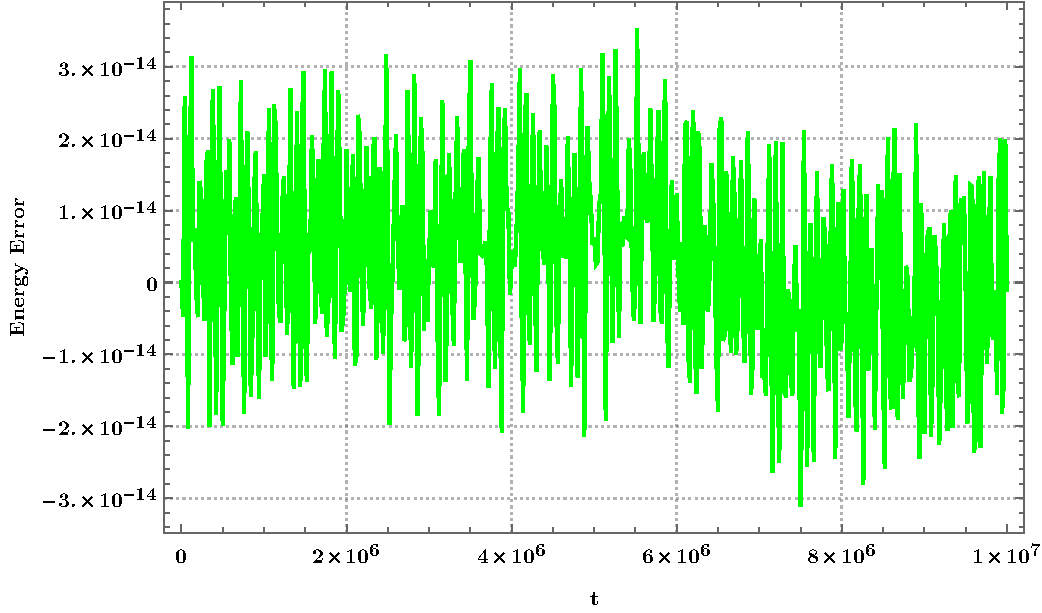
\includegraphics[width=.4\textwidth]{Fig2}}
&
\subfloat[$k=0$ energia errorearen desbideratze estandarra]
{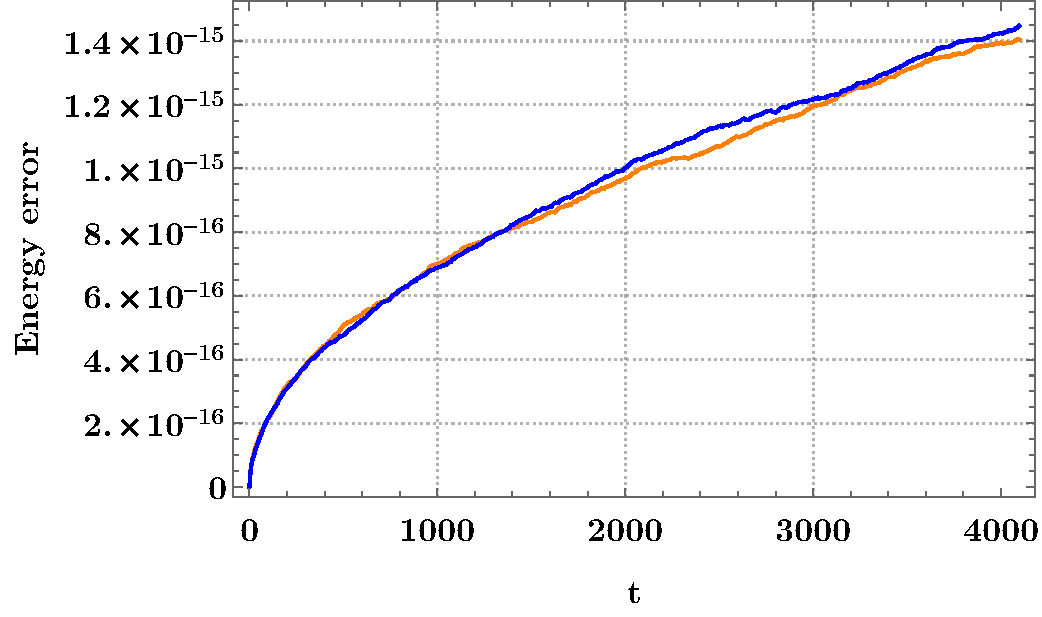
\includegraphics[width=.4\textwidth]{Fig3}}
\\
\subfloat[$k=2^{10}$ energia errorrearen batezbestekoa]
{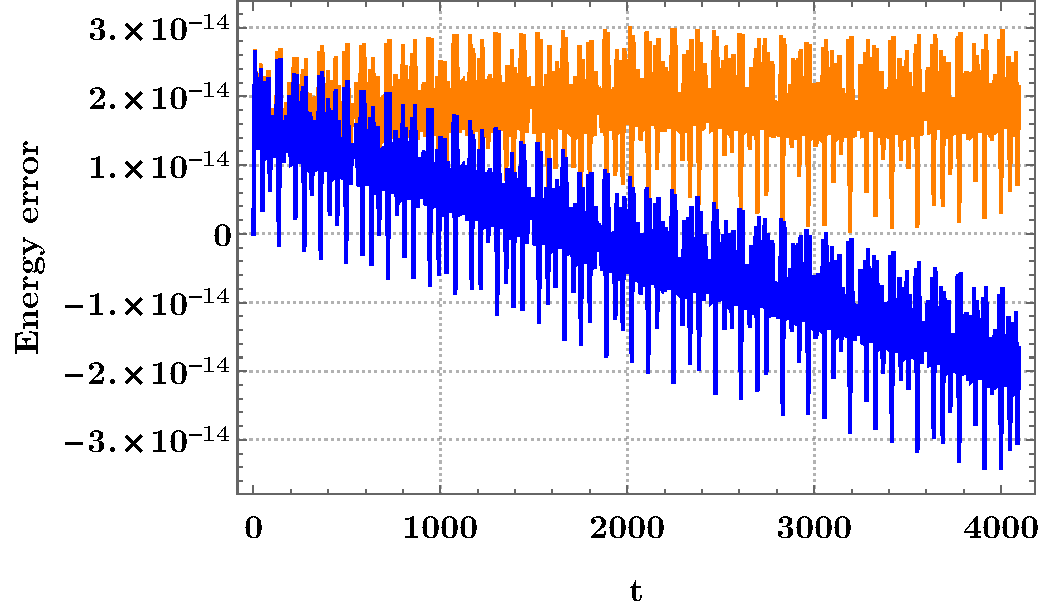
\includegraphics[width=.4\textwidth]{Fig4}}
&
\subfloat[$k=2^{10}$ energia errorearen desbideratze estandarra]
{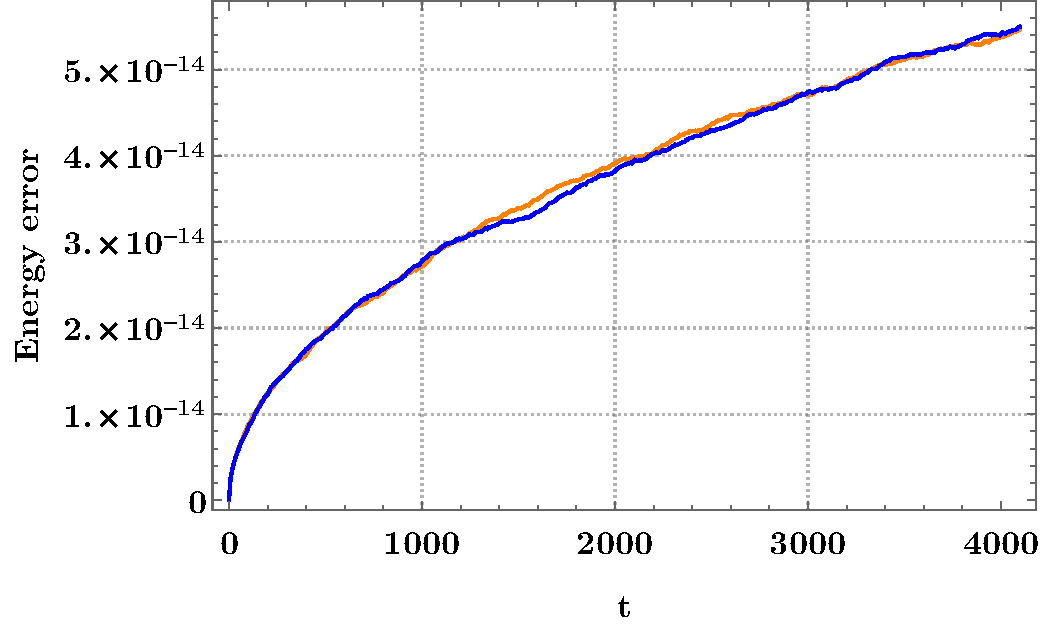
\includegraphics[width=.4\textwidth]{Fig5}}
\\
\subfloat[$k=2^{12}$ energia errorrearen batezbestekoa]
{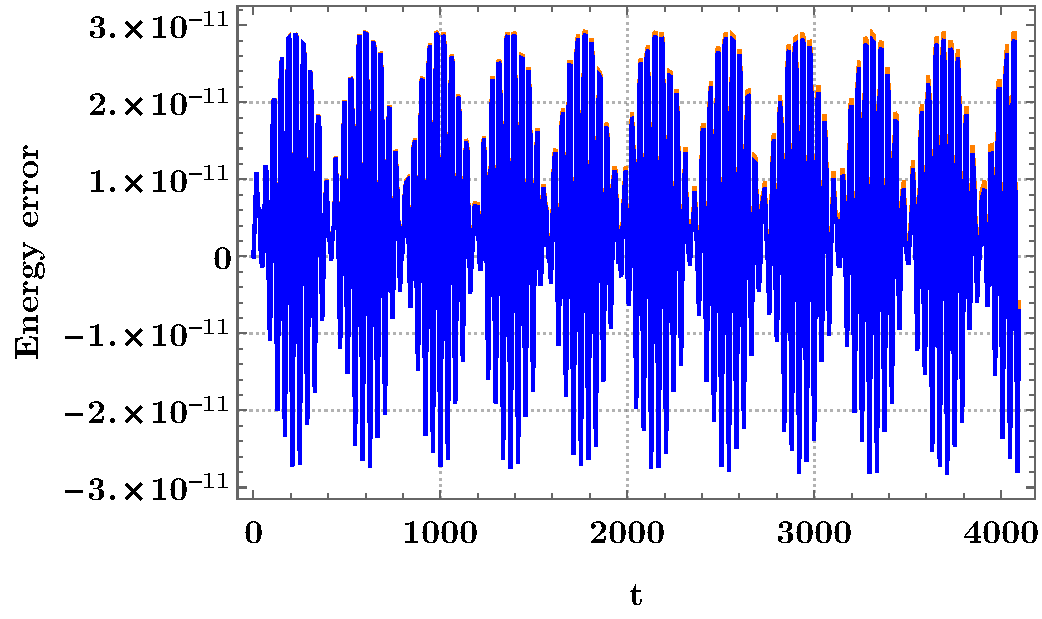
\includegraphics[width=.4\textwidth]{Fig6}}
&
\subfloat[$k=2^{12}$ energia errorearen desbideratze estandarra]
{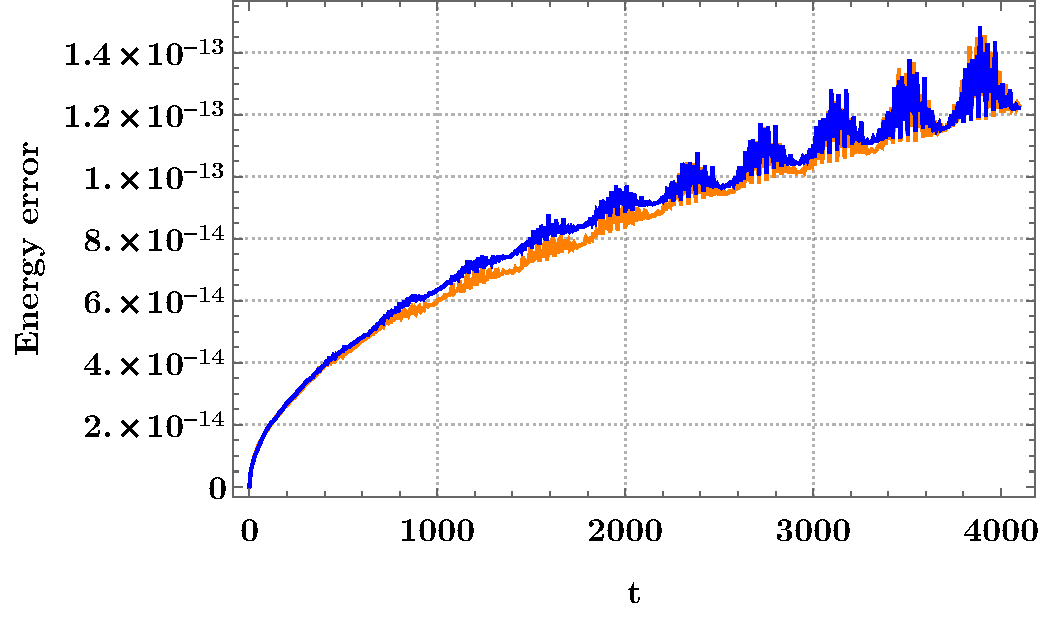
\includegraphics[width=.4\textwidth]{Fig7}}
\end{tabular}
\caption{\small Energia errore batezbestekoaren (ezkerrean) eta desbideratze estandarraren  eboluzioa (eskubian), puntu-finkoaren inplementazioa (urdinez), eta  Newton inplementazioa (laranjaz). $k=0$ problema ez-zurruna (a,b), $k=2^{10}$ lehen problema zurruna (c,d) eta $k=2^{12}$ bigarren problema zurruna (e,f)}
\label{fig:plot3}
\end{figure}


\subsection{Puntu-finkoa versus Newton iterazioa}


\ref{tab:fp1} taulan, $k$ parametroaren lau balioetarako, bi inplementazioen eraginkortasunaren adierazle nagusienak laburtu ditugu.

\begin{table}[h!]
\caption[Fixed-point percentage of steps and mean iterations.] 
{}
\label{tab:fp1}       % Give a unique label
\centering
{%
\begin{tabular}{ l l l l l } 
 \hline
%                 &  \multicolumn{2}{c}{FPIEA}  & \multicolumn{2}{c}{DP} & \multicolumn{2}{c}{Hairer} \\
\\
 C               & $0$  & $2^3$ & $2^6$ & $2^8$ \\
 $E_0$           & $-14.39$  & $-5.75$ & $-5.64$ & $-5.64$ \\ 
\\
 \hline
\\
 Fixed-points it.&           &         &         &         \\
 \cline{1-1}     &           &         &         &         \\
 Elapsed-time (sec.)    & $10$      & $12$    & $19$    & $51$    \\ 
 It. per step    & $8.58$    & $11.1$  & $22.$  & $64.2$  \\
 Energy          & $2.96\times 10^{-15}$ & $1.81\times 10^{-14}$ & $2.94\times 10^{-11}$ & $6.33\times 10^{-5}$ \\
 \\
 Newton it.            &           &         &         &         \\
 \cline{1-1}           &           &         &         &         \\
 Elapsed-time (sec.)   & $18$      & $20$    & $19$    & $18$     \\
 It. per step          & $5.09$    & $5.53$  & $5.58$  & $5.01$   \\
 L. solves per step    & $11.37$   & $12.92$  & $12.72$  & $11.04$ \\
 Energy                & $1.6\times 10^{-15}$ & $1.74\times 10^{-14}$ & $2.94\times 10^{-11}$ & $6.33\times 10^{-5}$ \\   
 \\  
   \hline
 \end{tabular}}
\end{table}

Eraginkortasuna neurtzeko, bi inplementazioen exekuzio sekuentzialen cpu-denborak  konparatu ditugu. Hortaz gain, bi inplementazioen urratseko iterazio batezbestekoak (It. per step) alderatu ditugu eta Newton inplementazioan, urratseko sistema linealen ebazpen batezbestekoa (L.solves per step) eman dugu. Zenbakizko soluzioaren doitasuna neurtzeko, energia errore erlatibo maximoa eman dugu,
\begin{equation*}
\max | \frac{E(t_n)-E(t_0)}{E(t_0)} |, \ \  t_n=t_0+nh, \ \ n=1,2,\dots
\end{equation*} 

$k$ balio txikienetarako, puntu-finkoaren inplementazioa Newton inplementazioa baino eraginkorragoa da. Baina, pendulu bikoitzaren zurruntasun maila handitzen dugunean, puntu-finkoaren iterazio kopurua gero eta handiagoa den bitartean, Newton inplementazioaren iterazio kopurua zerbait txikiagoa da $k$ balio handienetarako. Beraz, zurruntasuna handitzen dugunean, Newton inplementazioa gero eta eraginkorragoa bilakatzen da. $k=2^{18}$ baliotik aurrera, puntu-finkoak ez du konbergitzen eta Newton inplementazioak, iterazio kopuru antzekoarekin konbergitzen du.

 
%\small{Percentage of steps that reach a computational fixed-point and the number of fixed-point iterations per step for the computations of  double pendulum stiff problem}



\section{Laburpena.}


